\documentclass[xcolor=dvipsnames, 14pt]{beamer}
%\documentclass[xcolor=dvipsnames, bigger, aspectratio=169]{beamer}

\definecolor{Saffron}{HTML}{F4C430}
\usecolortheme[named=Saffron]{structure}

\mode<presentation> {
	\usetheme[height=2em]{Rochester}
	\setbeamercovered{transparent}
}

\setbeamertemplate{caption}{\insertcaption\par}
\setbeamertemplate{navigation symbols}{}%remove navigation symbols

\setbeamercolor{frametitle}{fg=black}
\setbeamercolor{title}{fg=black}
\setbeamercolor{navigation symbols dimmed}{fg=black!10}
\setbeamercolor{navigation symbols}{fg=black!30}
\setbeamercolor{section number projected}{fg=black}
\setbeamercolor{item projected}{fg=black}


\usepackage[utf8x]{inputenc}
\usepackage[resetfonts]{cmap}
\usepackage{lmodern}
\usepackage[english]{babel}
\usepackage[T1]{fontenc}

\usepackage{graphicx}
\usepackage{amsmath}
\usepackage{amssymb}
\usepackage{listings}
\usepackage{microtype}
\usepackage{tikz}

\usepackage{hyperref}
\hypersetup{unicode=true}

% ----- macros -----
\newcommand{\imageW}[1]{%
  \makebox[\textwidth][c]{\includegraphics[width=1.12\textwidth]{img/#1}}}
\newcommand{\imageH}[1]{%
  \makebox[\textwidth][c]{\includegraphics[height=0.86\textheight]{img/#1}}}

% ---- info -----
\title{Adaptive Programming}
\author{Jaroslav~Čechák \and Tomáš~Effenberger \and  Jiří~Mauritz \and Jakub Peschel}
\institute{Faculty of Informatics, Masaryk University}
\date{\today}

\begin{document}

\begin{frame}
\titlepage
\end{frame}

\begin{frame}
\frametitle{Goal}
TODO (both long term and short term goal = within RecSys course)
\end{frame}

\begin{frame}
\frametitle{Flow}
\begin{figure}[h]
  \centering
  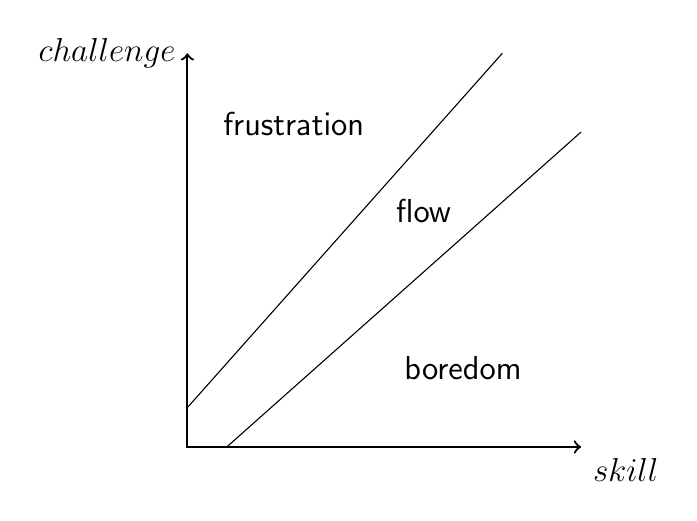
\begin{tikzpicture}[font=\sffamily,xscale=5, yscale=5]
  \large
  %\draw [lightgray, fill=gray] (0,0) -- (0.1,0) -- (1,0.8) -- (0.8,1) -- (0,0.1) -- (0,0);
  \draw (0.1,0) -- (1,0.8);
  \draw (0,0.1) -- (0.8,1);
  \draw [thick, <->] (0,1) node [left] {$challenge$} -- (0,0) -- (1,0) node [below right] {$skill$};
  \node at (0.27,0.82) {frustration};
  \node at (0.6,0.6) {flow};
  \node at (0.7,0.2) {boredom};
  \end{tikzpicture}
  %\caption{Relationship between challenge and skill.}
\end{figure}
\end{frame}

\begin{frame}
\frametitle{Existing projects and research}
TODO (this can be similar to what we prepared for the ALG seminar, but should be brief)
\end{frame}

\begin{frame}
\frametitle{Developed prototype}
\imageW{easy-task-initial.png}
\end{frame}

\begin{frame}
\frametitle{Developed prototype}
\imageW{easy-task-program.png}
\end{frame}

\begin{frame}
\frametitle{Developed prototype}
\imageW{easy-task-solved.png}
\end{frame}

\begin{frame}
\frametitle{Developed prototype}
\imageW{task-loops-initial.png}
\end{frame}

\begin{frame}
\frametitle{Developed prototype}
\imageW{complex-program.png}
\end{frame}

\begin{frame}
\frametitle{Developed prototype}
\imageW{task-colors.png}
\end{frame}

\begin{frame}
\frametitle{Developed prototype}
\imageW{task-keys.png}
\end{frame}

\begin{frame}
\frametitle{Developed prototype}
\imageW{task-pits.png}
\end{frame}

\begin{frame}
\frametitle{Models}
TODO: model of student skills and task difficulty
\end{frame}

\begin{frame}
\frametitle{Tasks}
TODO: details about tasks, incl.generating initial difficulty
\begin{itemize}
\item initial task difficulty generated
% note: what information are we using to generate initial difficulty (number of concepts, number of blocks, plan size, number of free fields, number of tokens, block limit)
\end{itemize}
\end{frame}

%\begin{frame}
%\frametitle{Initial tasks difficulty}
%\small
%\begin{equation*}
%\begin{split}
%  \mbox{diff}(t) = & \tanh ((b_t - K_1) + (5 m - K_2) + (5 l_t - K_3) \\
%                   & + 0.5\ln{(f)}) / K_{13}) \\
%                   & + K_8 (c_t - K_8)
%\end{split}
%\end{equation*}
%\end{frame}

\begin{frame}
\frametitle{Prediction}
TODO: how we predict flow
\end{frame}

\begin{frame}
\frametitle{Task selection}
TODO: how we select the best task
\end{frame}

\begin{frame}
\frametitle{Parameters update}
TODO: 2 phases: (1) update based on report, (2) learning shift
\end{frame}

\begin{frame}
\frametitle{Simulations}
TODO: plots of normal, stupid, genius students..
\end{frame}

\begin{frame}
\frametitle{Implementation}
TODO: implementation details (overview + interesting parts)
\end{frame}

\begin{frame}
\frametitle{Evaluation}
\begin{itemize}
\item not enough data
\end{itemize}
TODO: (at least we can show some basic statistics and how the task difficulties changed in time)
\end{frame}

\begin{frame}
\frametitle{Experience report}
TODO: present experience reports from users
\end{frame}

\begin{frame}
\frametitle{Summary}
\begin{itemize}
\item system for adpative learning of programming
\item Blockly language, tasks in a maze
\item concept of flow, Elo model
\item first prototype: link
\item source codes: link
\end{itemize}
\end{frame}

\end{document}
